\chapter{Technical approach}

The proposed two-stream approach consists of an appearance
stream, representing the static (texture) appearance of each frame,
and a dynamics stream, representing temporal 
variations between frames.
Each stream consists of a ConvNet whose activation 
statistics are used to characterize the dynamic texture.
Synthesizing a dynamic texture is formulated as an optimization 
problem with the objective of matching these activation 
statistics.
The dynamic texture synthesis approach is summarized in Fig.\ \ref{fig:architecture}
and the individual pieces are described in turn in the
following sections.

\begin{figure}[t]
\begin{center}
    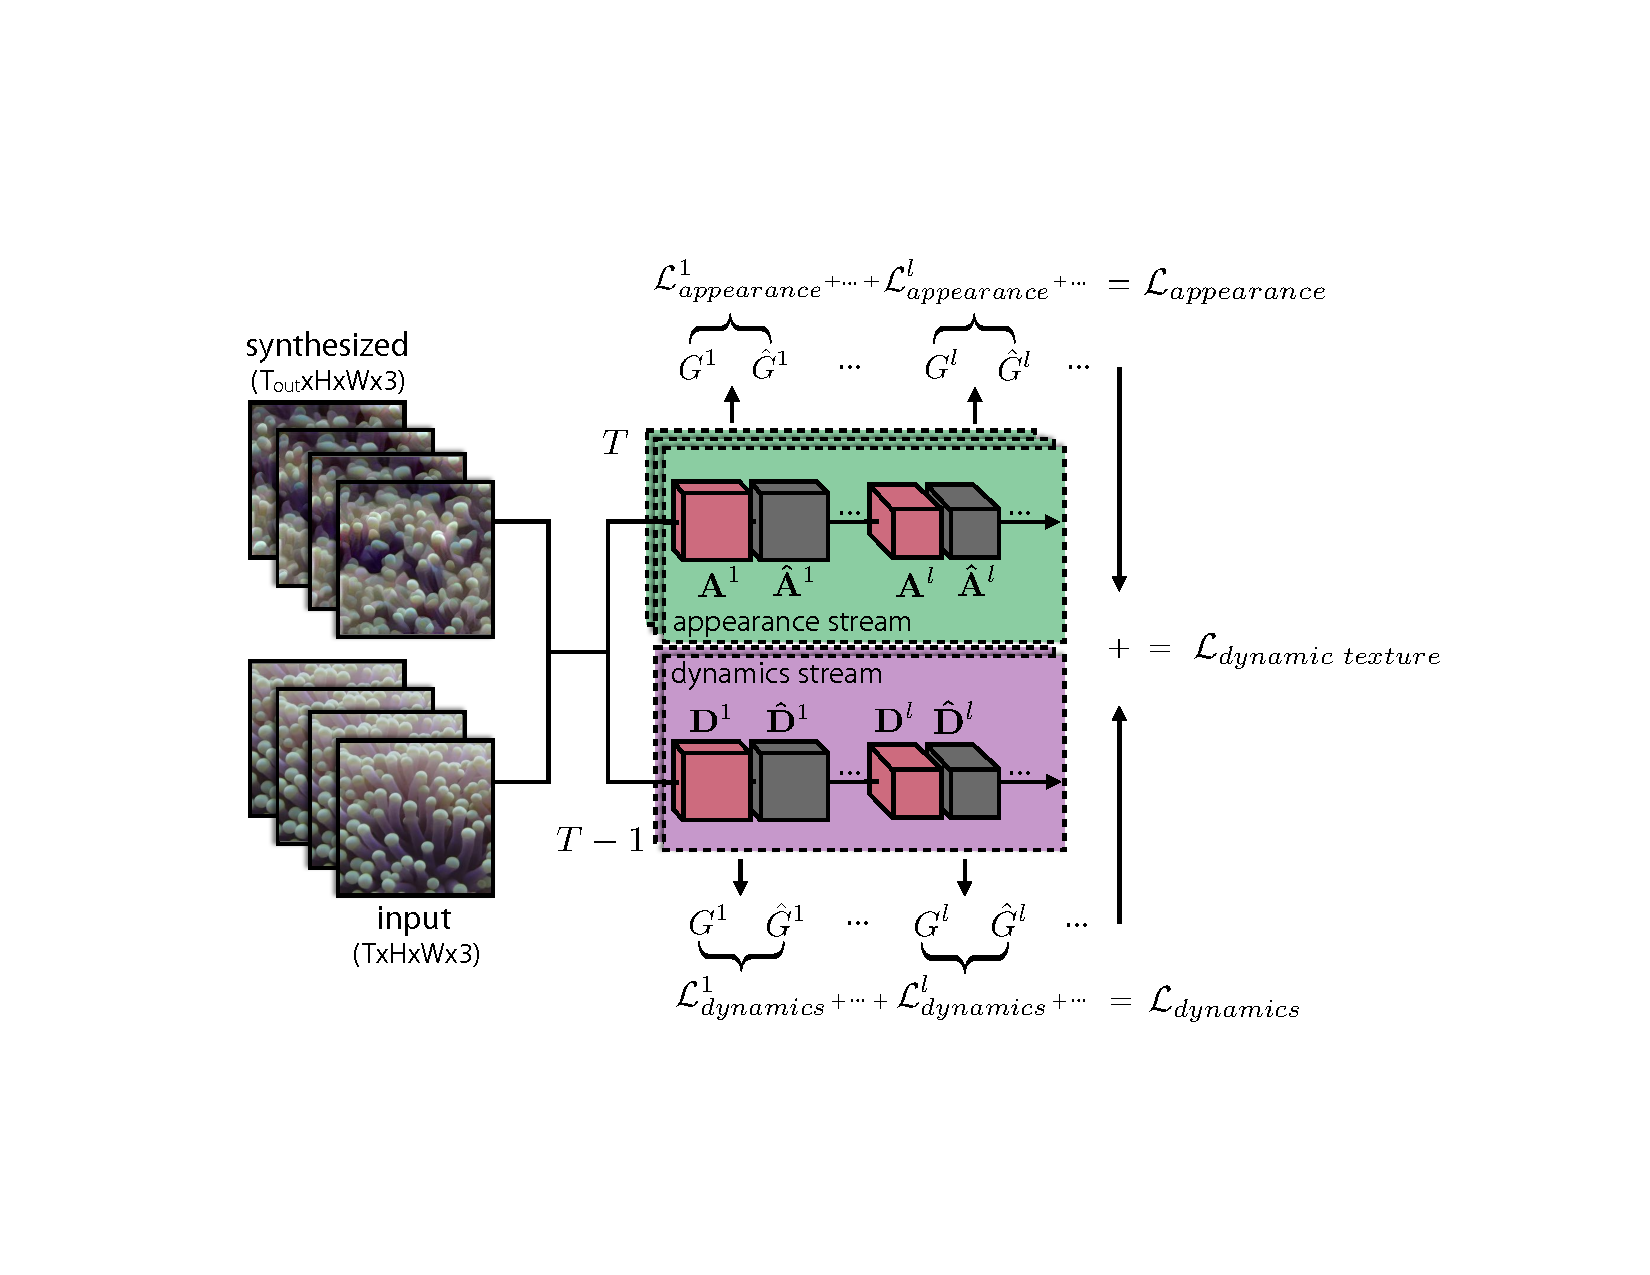
\epsfig{file=overallarchitecture.pdf, width = \textwidth}
\end{center}
\vspace{-0.45cm}
\caption[Two-stream dynamic texture generation.]{Two-stream dynamic texture generation.
Two sets of Gram matrices represent a dynamic texture's appearance and 
dynamics.
Matching these statistics allows for the generation of novel
textures as well as style transfer between textures. Here, $G^l$ and $\hat{G}^l$ are the Gram matrices of activations $A^l$ and $\hat{A}^l$ (or $D^l$ and $\hat{D}^l$) corresponding to the target and synthesized sequence, respectively, computed at layer $l$ of the appearance stream (or dynamics stream) and averaged over time $T$ (or $T-1$). $\mathcal{L}_\text{appearance}^l$ is the appearance loss at layer $l$, computed as the squared Frobenius norm between $G^l$ and $\hat{G}^l$ from the appearance stream. Similarly, $\mathcal{L}_\text{dynamics}^l$ is the dynamics loss at layer $l$ for the dynamics stream. By summing each loss computed at various layers, we arrive at $\mathcal{L}_\text{appearance}$ and $\mathcal{L}_\text{dynamics}$, which, when summed, form the combined dynamic texture loss, $\mathcal{L}_\text{dynamic texture}$, that is to be minimized.}
\label{fig:architecture}
\end{figure}


\section{Texture model: Appearance stream}

The appearance stream follows the spatial texture model
introduced by Gatys \etal \cite{gatys2015} which was reviewed in the previous chapter \todomatthew{talk about Gatys style transfer in related work}.
\todomatthew{talk about texture synthesis in related work}
To briefly review, the key idea is that feature auto-correlations (\ie, normalized \emph{Gram} matrices) in a 
ConvNet trained for 
object recognition (\eg, VGG-19 \cite{simonyan2014very}) 
capture texture appearance.
The same publicly available normalized VGG-19 ConvNet \cite{simonyan2014very} used by Gatys \etal \cite{gatys2015} is used here.

\subsection{Target texture appearance}

To capture the appearance of an input dynamic texture, an initial forward pass through VGG-19 is performed with each frame of the image sequence to compute the feature activations (filter responses),
$\mathbf{A}^{lt} \in \mathbb{R}^{N_l\times M_l}$, for various
levels in the network, where $N_l$ and $M_l$ denote
the number of feature activations and the number of spatial locations of layer
$l$ at time $t$, respectively.
The auto-correlations of the filter responses in a particular layer are
averaged over the frames and encapsulated by a Gram matrix,
$\mathbf{G}^{l} \in \mathbb{R}^{N_l \times N_l}$, whose
entries are given by:
\begin{equation}
	G_{ij}^l = \frac{1}{T N_l M_l} \sum_{t=1}^T \sum_{k=1}^{M_l} A_{ik}^{lt} A_{jk}^{lt}\ ,
	\label{eq:gram_target}
\end{equation}
where $T$ denotes the number of input frames
and $A_{ik}^{lt}$ denotes the activation of feature $i$ at
location $k$ in layer $l$ on the target frame $t$.

\subsection{Synthesized texture appearance}

The synthesized texture appearance is similarly represented by a
Gram matrix, $\hat{\mathbf{G}}^{lt} \in \mathbb{R}^{N_l \times N_l}$,
whose activations are given by:
\begin{equation}
	\hat{G}_{ij}^{lt} = \frac{1}{N_l M_l} \sum_{k=1}^{M_l} \hat{A}_{ik}^{lt} \hat{A}_{jk}^{lt}\ ,
	\label{eq:gram_synthesized}	
\end{equation}
where $\hat{A}_{ik}^{lt}$ denotes the activation of feature $i$ at
location $k$ in layer $l$ on the synthesized frame $t$.

\subsection{Appearance loss}

The appearance loss, $\mathcal{L}_\text{appearance}$, is then 
defined as the temporal average of the mean squared error between
the Gram matrix of the input texture and that of the synthesized
texture computed at each frame:
\begin{equation}
   \mathcal{L}_\text{appearance} = \frac{1}{L_\text{app} T_\text{out}} \sum_{t=1}^{T_\text{out}} \sum_{l} \Vert \mathbf{G}^l - \hat{\mathbf{G}}^{lt} \Vert^2_F\ ,
   \label{eq:apploss}
\end{equation}
where $L_\text{app}$ is the number of VGG-19 layers used to compute Gram
matrices, $T_\text{out}$ is the number of frames being generated in
the output, and $\Vert \cdot \Vert_F$ is the Frobenius norm.
Consistent with previous work \cite{gatys2015}, Gram matrices are computed on the
following layers: 
\emph{conv1\_1}, \emph{pool1}, \emph{pool2}, \emph{pool3}, and \emph{pool4}.

\section{Texture model: Dynamics stream}

There are three primary goals in designing the dynamics stream ConvNet.
\begin{enumerate}
	\item The activations of the ConvNet must represent the temporal variation of the input pattern.
	\item The activations should be largely invariant to the appearance (\ie, spatial content) of the images (which should be characterized by the appearance stream described above).
	\item The dynamics representation must be differentiable to enable synthesis via a ConvNet.
\end{enumerate}

By analogy to the appearance stream, an obvious choice
is a ConvNet architecture suited for computing
optical flow \todomatthew{talk about optical flow in related work} (\eg, \cite{dosovitskiy2015,ilg2017}) which
is naturally differentiable.
However, with most such models it is unclear how invariant
their layers are to appearance.
Instead, a novel network architecture is proposed which is
motivated by the spacetime-oriented energy model
\cite{derpanis2012spacetime,simoncelli1998}. \todomatthew{talk about SOE for texture recognition in related work?}

\subsection{Review: Marginalized spacetime oriented energies}

In motion energy models, the velocity of image content (\ie, motion)
is interpreted as a 3D orientation in the $x$-$y$-$t$
spatiotemporal domain
\cite{adelson1985spatiotemporal,fahle1981,heeger1988,simoncelli1998,watson1983}. \todomatthew{include figure of motion in xyt}
In the frequency domain, the signal energy of a translating
pattern can be shown to lie on a plane through the origin
where the slant of the plane is defined by the velocity of
the  pattern. \todomatthew{include figure of motion in frequency space}
Thus, motion energy models attempt to identify this 
orientation-plane (and hence the pattern's velocity) via
a set of image filtering operations.
More generally,
the constituent
spacetime orientations for a spectrum of common
visual patterns can serve as a basis for describing the temporal
variation of an image sequence \cite{derpanis2012spacetime}.
This observation suggests that motion energy models may form an
ideal basis for the dynamics stream. Specifically, the spacetime-oriented energy models proposed by Derpanis \etal \cite{derpanis2012spacetime}
and Simoncelli \etal \cite{simoncelli1998} are used to motivate the
network architecture, which is briefly reviewed here; 
see Chapter \ref{chap:background} \todomatthew{talk about Derpanis' MSOE in related work} for a more in-depth description.

Given an input video, 
a bank of oriented 3D
filters, which are sensitive to a range of
spatiotemporal orientations, are applied.
These filter activations are then rectified (squared) and
pooled over local regions to make the responses robust
to the phase of the input signal, \ie, robust to the
alignment of the filter with the underlying image
structure. At this point, each oriented energy measurement is confounded with spatial orientation. Consequently, in cases where the 
spatial image structure varies wildly about an otherwise coherent dynamic
region, the responses of the bank of oriented filters will reflect this
behaviour and thereby become dependent on spatial appearance; whereas, a description consisting purely 
of pattern dynamics is sought.
To remove this difficulty, the spatial orientation component of each filter is discounted via ``marginalization''. Specifically, filter activations consistent with the same temporal orientation (not necessarily the same spatial orientation) are summed. \todomatthew{clarify with Kosta}
These responses provide a pixelwise distributed measure
of which orientations (frequency domain planes) are
present in the input.
However, these responses are confounded by local image
contrast that makes 
it difficult to determine
whether a high response is indicative of the presence of
a spacetime orientation or simply due to high image
contrast.
To address this ambiguity, an $\textrm{L}_1$
normalization is applied across orientation responses which
results in a representation that is robust to local
appearance variations but highly selective to 
spacetime orientation.

\subsection{ConvNet architecture}

Using this model as the basis, the following fully convolutional 
network \cite{shelhamer2017} \todomatthew{talk about this in related work?} is proposed.
The ConvNet input is a pair of temporally consecutive greyscale images, $\mathbf{I} \in \mathbb{R}^{T \times H \times W \times C}$ ($\text{time} \times \text{height} \times \text{width} \times \text{channels}$), where $C=1$ and $T=2$. From here forth, the channel dimension ($C$) will be omitted for simplicity.
Each input pair is first normalized to have zero-mean and unit
variance (\ie, contrast normalization or ``instance normalization'' \cite{ulyanov2017}), as follows:
\begin{equation}
	\mathbf{I}_N = \frac{\mathbf{I} - \mu}{\sigma + \epsilon}\ ,
\end{equation}
where $\mu$ is the average pixel value of the input pair, $\sigma$ is the standard deviation of the input pair, and $\epsilon$ is a small value to prevent dividing by zero.
This step provides a level of invariance \todomatthew{Rick: Given that you're using normalized, bandpass filters, is this preprocessing necessary?} to overall brightness and contrast, \ie, global additive and
multiplicative signal variations, easing the training process of the ConvNet. \todomatthew{maybe talk about how it relates to batchnorm?}
The first layer consists of a 3D convolution over the normalized input pair with a bank of 32 3D filters of size $2 \times 11 \times 11$
($\text{time} \times \text{height} \times \text{width}$), resulting in an output of spacetime oriented energy measurements, \todomatthew{Rick: Really only 2 taps in time?}
\begin{equation}
	E_F(\mathbf{x}) = F * \mathbf{I}_N(\mathbf{x})\ ,
\end{equation}
where $E_F$ denotes the response of filter $F$ (of size $2 \times 11 \times 11$) after a convolution, $*$, centered about $\mathbf{x} \equiv (t, x, y)$.
Next, a squaring activation function and $5 \times 5$
spatial max-pooling (with a stride of one) is applied to
make the responses robust to local signal phase:
\begin{equation}
	\bar{E}_F(\mathbf{x}) = \max_{i\in\Omega}\{E_F(i)^2\}\ ,
\end{equation}
where $\Omega$ is a $5 \times 5$ spatial neighbourhood centered about $\mathbf{x}$.
A 2D convolution follows with 64 filters of size $1 \times 1$ that combines
energy measurements that are consistent
with the same orientation:
\begin{equation}
	E_G(\mathbf{x}) = G * \bar{E}_F(\mathbf{x})\ ,
\end{equation}
where  $E_G$ denotes the response of filter $G$ (of size $1 \times 1$) after a convolution.
Finally, to remove local contrast dependence, an
$\text{L}_1$ divisive normalization is applied to each spatial location: \todomatthew{explain why this is not redundant due to contrast norm on input}
\begin{equation}
	\bar{E}_G(\mathbf{x}) = \frac{E_G(\mathbf{x})}{\Vert E_G(\mathbf{x}) \Vert_1 + \epsilon}\ ,
\end{equation}
where $\Vert \cdot \Vert_1$ is the $\text{L}_1$ norm computed over the filter responses of all filters.

To capture spacetime orientations beyond those capable
with the limited receptive fields used in the initial
layer, a five-level spatial Gaussian pyramid is computed.
Each pyramid level is processed independently
with the same spacetime-oriented energy model and then
bilinearly upsampled to the original resolution and
concatenated:
\begin{equation}
	E(\mathbf{x}) = \left( \bar{E}_G(\mathbf{x}) \Vert \bar{E}_G(\mathbf{x}_{\downarrow\times2})_{\uparrow\times2} \Vert \cdots \Vert \bar{E}_G(\mathbf{x}_{\downarrow\times2^{k-1}})_{\uparrow\times2^{k-1}} \Vert \bar{E}_G(\mathbf{x}_{\downarrow\times2^k})_{\uparrow\times2^k} \right)\ ,
\end{equation}
where $(\cdot)_{\downarrow \times n}$ and $(\cdot)_{\uparrow \times n}$ denote an $n$-times downsample and upsample, respectively, and $k+1$ denotes the number of pyramid levels. This final output of the dynamics encoding stage is named the ``concatenation layer''.

\subsubsection{Training}

Prior energy model instantiations (\eg,
\cite{adelson1985spatiotemporal,derpanis2012spacetime,simoncelli1998})
used handcrafted filter weights.
While a similar approach could be followed here, instead the weights
are learned so that they better deal with the noise distributions encountered in natural imagery.
To train the network weights, additional decoding
layers are added that take the concatenated distributed
representation from the concatenation layer and apply a $3\times 3$ convolution
(with 64 filters), ReLU activation, and a $1\times 1$
convolution (with 2 filters) that yields a two channel
output encoding the optical flow directly. \todomatthew{introduce optical flow in related work as background}
The proposed architecture is illustrated in
Fig.\ \ref{fig:MSOE}.

\begin{figure}[t]
\begin{center}
    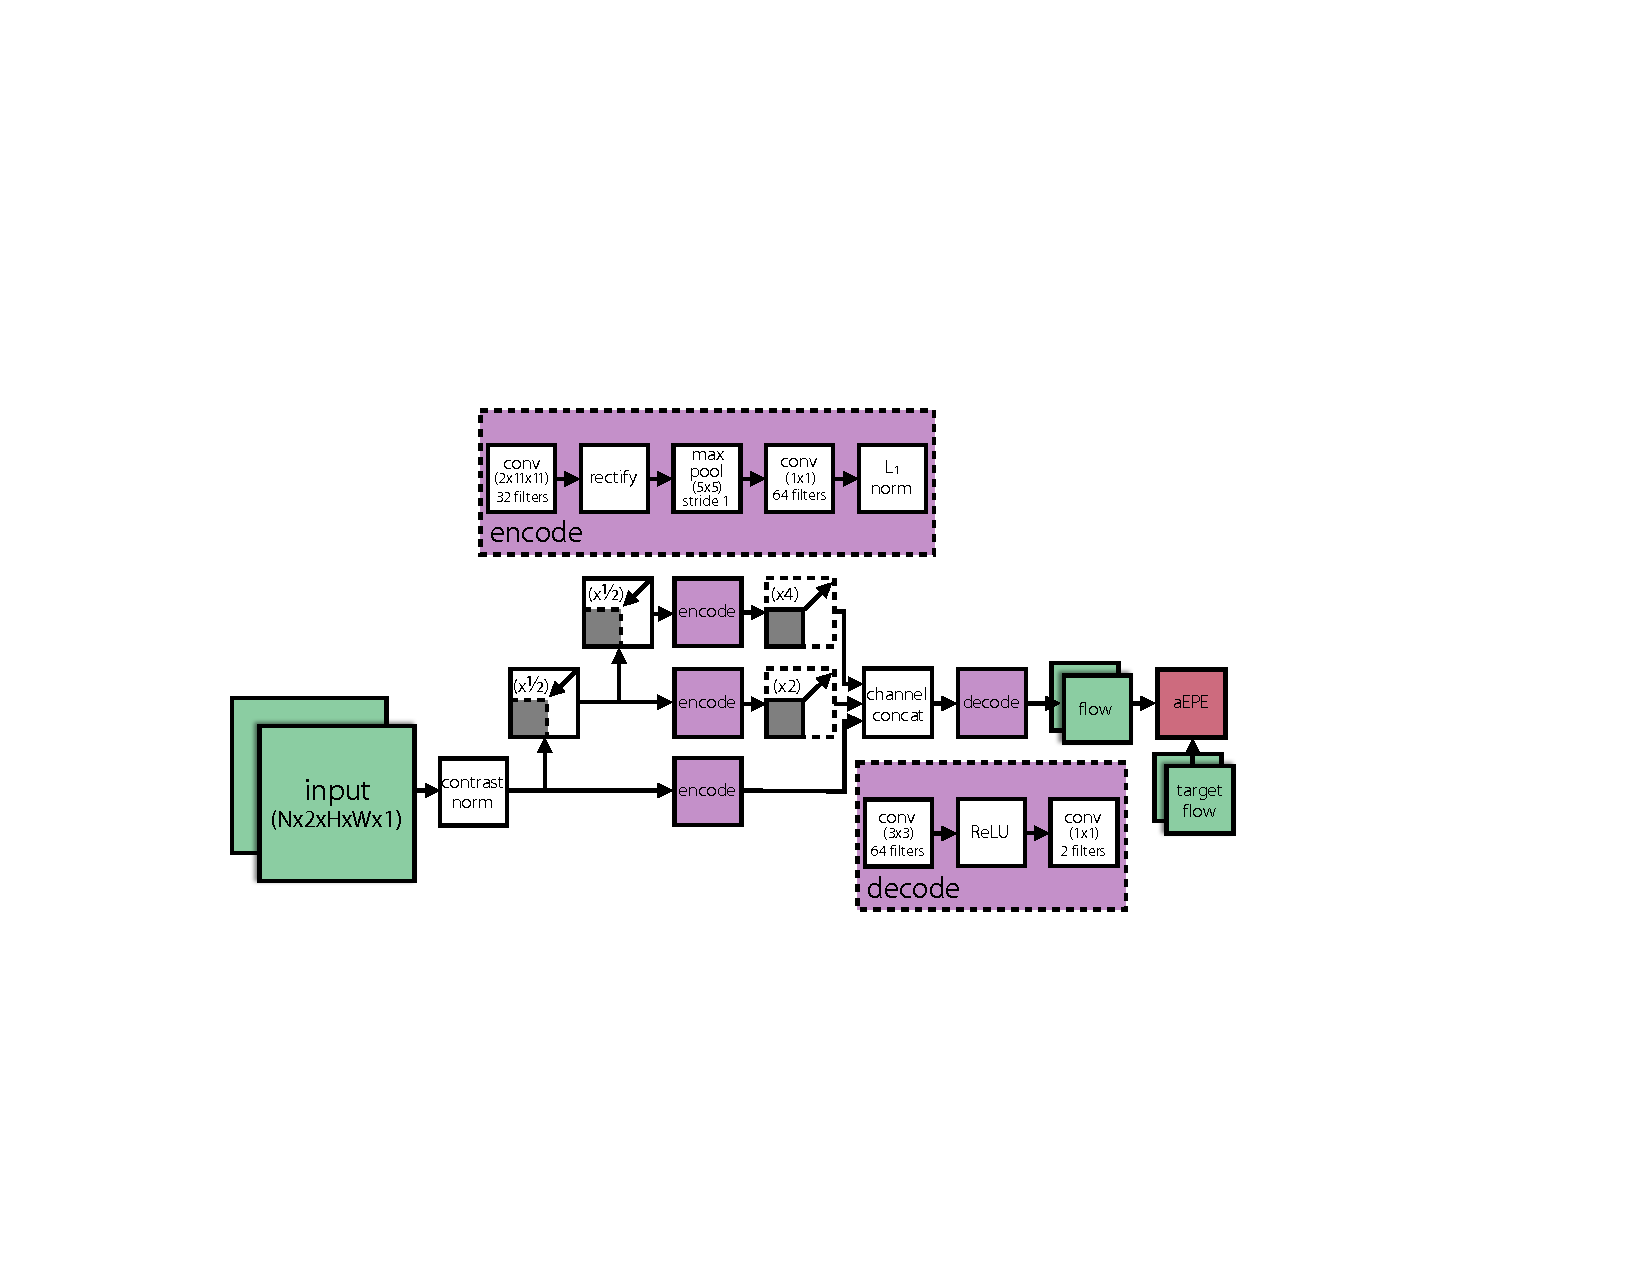
\epsfig{file=MSOEnet.pdf, width = \textwidth}
\end{center}
\vspace{-0.45cm}
\caption[Dynamics stream ConvNet.]{Dynamics stream ConvNet. The ConvNet is based on a
spacetime-oriented energy model
\cite{derpanis2012spacetime, simoncelli1998} and is trained
for optical flow prediction.
Three scales are shown for illustration;
in practice five scales are used.}
\label{fig:MSOE}
\end{figure}

For training, the standard average
endpoint error (aEPE) flow metric (\ie, $\text{L}_2$
norm) is used between the predicted flow and the ground truth
flow as the loss.
Since no large-scale optical flow dataset exists that captures
natural imagery with groundtruth flow, a new dataset had to be made. Videos
from an unlabeled video dataset are fed through an existing flow
estimator to produce optical
flow ``semi-groundtruths'' for training,
\cf \cite{tran2016}.
For the unlabeled video dataset, the UCF101
dataset for action recognition \cite{soomro2012ucf101} is used as it contains complex movements of natural imagery at desirably slow speeds \todomatthew{histogram of flow magnitudes}, similar to the expected pattern velocity of the dynamic textures used in this work. The synthetic Flying Chairs dataset \cite{dosovitskiy2015} was also considered as it contained ground truth optical flow, however, training the dynamics stream on this dataset reduced the overall quality of synthesized dynamic textures. This can be explained by the less complex and faster movement of the rigid objects in Flying Chairs, which is undesirable for estimating motion of dynamic textures.
For producing the optical flow semi-groundtruths, a ConvNet-based model, EpicFlow \cite{revaud2015epicflow}, is used for 
its superior performance over traditional handcrafted approaches and tendency
to produce smooth predictions---ideal training data for the dynamics stream. \todomatthew{talk about why EpicFlow and not FlowNet?}

The distribution of movement directions \todomatthew{radial histogram of flow for ucf101} in UCF101 is biased to left-to-right and right-to-left motions, which is undesirable as dynamic textures are not necessarily restricted to certain directions of motion. To combat this dataset bias, geometric data augmentations \todomatthew{provide geo augmentations} similar to those used by FlowNet \cite{dosovitskiy2015} are used to equalize the distribution of movement directions in the generated dataset. Additionally, photometric data augmentations \todomatthew{provide photo augmentations} similar to those used by FlowNet \cite{dosovitskiy2015} are used here as well. The aEPE loss is optimized using Adam \cite{kingma2017}.
Inspection of the learned filters in the initial layer of the encoding stage
showed evidence of spacetime-oriented filters, consistent with
the handcrafted filters used in previous work \cite{derpanis2012spacetime}. This is illustrated in Fig.\ \ref{fig:filters}.

\begin{figure}
	\centering
	\begin{subfigure}[b]{0.25\textwidth}
	    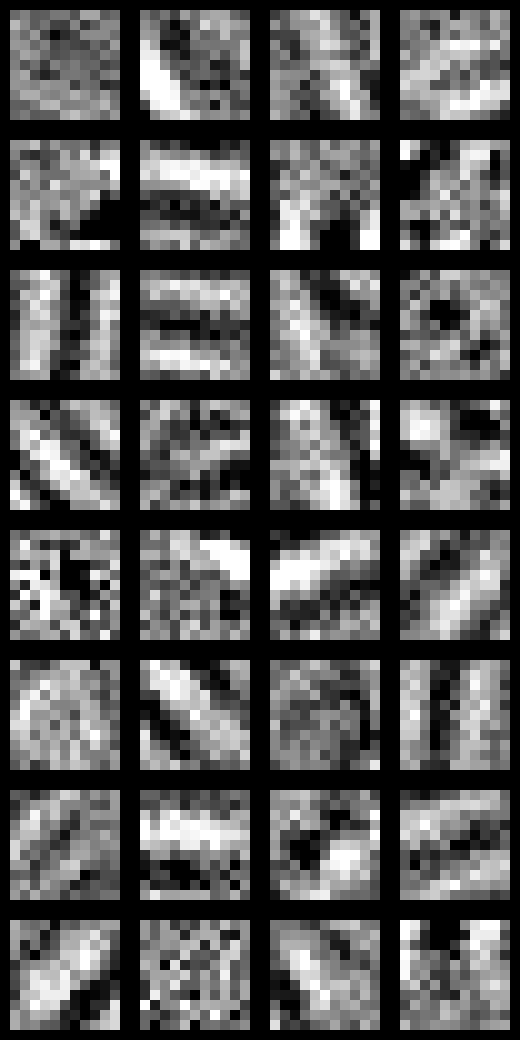
\epsfig{file=MSOEnet_filters_1.png, width = \textwidth}
		\vspace{-0.45cm}
		\caption{Frame 1}
	\end{subfigure}\hspace{5mm}%
	\begin{subfigure}[b]{0.25\textwidth}
	    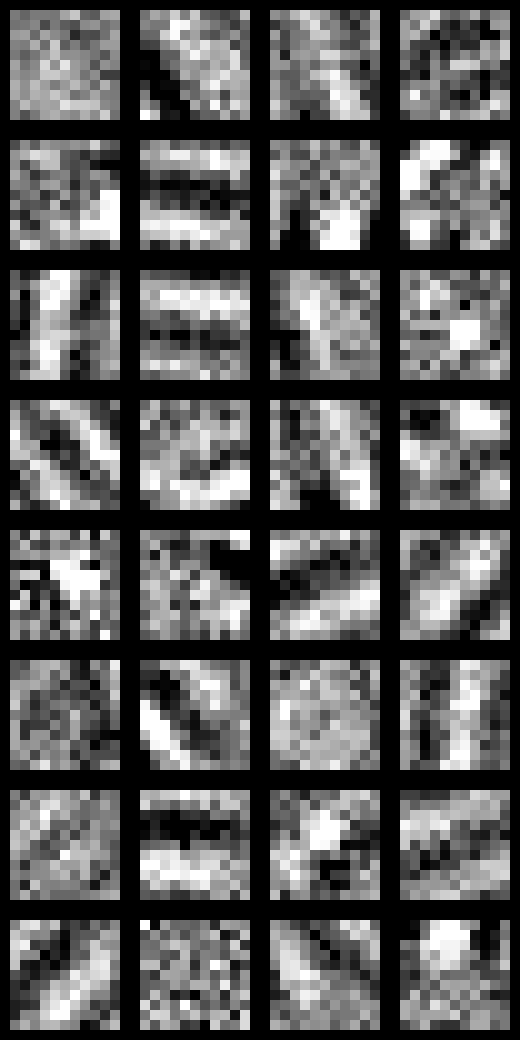
\epsfig{file=MSOEnet_filters_2.png, width = \textwidth}
		\vspace{-0.45cm}
		\caption{Frame 2}
	\end{subfigure}
	\caption[Learned spacetime-oriented filters]{32 learned spacetime-oriented filters of size $2 \times 11 \times 11$. (a) and (b) each depict a temporal slice of the learned filters, operating on the first and second frame of an input pair, respectively. Inspection of the learned filters reveals structures consistent with the handcrafted temporal derivative filters used in previous work \cite{derpanis2012spacetime} (\eg, row 4, col 1 captures up-right movement and row 8, col 1 captures down-right movement).}
	\label{fig:filters}
\end{figure}

\subsection{Target texture dynamics}

Similar to the appearance stream, filter response correlations
in a particular layer of the dynamics
stream are averaged over the number of image frame
pairs and encapsulated by a Gram matrix,
$\mathbf{G}^{l} \in \mathbb{R}^{N_l \times N_l}$,
whose entries are given by:
\begin{equation}
	G_{ij}^l = \frac{1}{(T-1) N_l M_l} \sum_{t=1}^{T-1} \sum_{k=1}^{M_l} D_{ik}^{lt} D_{jk}^{lt}\ ,	
\end{equation}
where $D_{ik}^{lt}$ denotes the activation of feature $i$ at
location $k$ in layer $l$ on the target frames $t$ and $t+1$.

\subsection{Synthesized texture dynamics}

The dynamics of the synthesized texture is represented
by a Gram matrix of filter response correlations 
computed separately for each pair of frames,
$\hat{\mathbf{G}}^{lt} \in \mathbb{R}^{N_l \times N_l}$,
with entries:
\begin{equation}
	\hat{G}_{ij}^{lt} = \frac{1}{N_l M_l} \sum_{k=1}^{M_l} \hat{D}_{ik}^{lt} \hat{D}_{jk}^{lt}\ ,	
\end{equation}
where $\hat{D}_{ik}^{lt}$ denotes the activation of feature $i$ at
location $k$ in layer $l$ on the synthesized frames $t$ and $t+1$.

\subsection{Dynamics loss}

The dynamics loss, $\mathcal{L}_\text{dynamics}$, is defined as
the average of the mean squared error between the Gram matrices
of the input texture
and those of the generated texture:
\begin{equation}
   \mathcal{L}_\text{dynamics} = \frac{1}{L_\text{dyn} (T_\text{out}-1)}\sum_{t=1}^{T_\text{out}-1} \sum_{l}  \Vert \mathbf{G}^l - \hat{\mathbf{G}}^{lt}\Vert^2_F, \label{eq:dynloss}
\end{equation}
where $L_\text{dyn}$ is the number of ConvNet layers being used
in the dynamics stream to compute Gram matrices.

The Gram matrix is computed on the output of the concatenation layer,
where the multiscale distributed representation of orientations is
stored. While it is tempting to use the predicted optical flow output from the
network's decoder stage, this generally yields poor results as shown in the evaluation.
Due to the complex, temporal variation present in dynamic
textures, they contain a variety of local spacetime
orientations rather than a single dominant orientation.
As a result, the flow estimates will tend to be an average of the
underlying  orientation measurements and consequently not
descriptive. A comparison between the texture synthesis results using the concatenation layer and the predicted flow output is provided in Chapter \ref{chap:evaluation}.

\section{Dynamic texture synthesis}\label{sec:texgen}
The overall dynamic texture loss consists of the combination of the appearance loss, Eq.\ (\ref{eq:apploss}),
and the dynamics loss, Eq.\ (\ref{eq:dynloss}):
\begin{equation}
   \mathcal{L}_\text{dynamic texture} = \alpha\mathcal{L}_\text{appearance} + \beta \mathcal{L}_\text{dynamics}, \label{eq:dyntexloss}
\end{equation}
where $\alpha$ and $\beta$ are the weighting factors for the
appearance and dynamics content, respectively.
Dynamic textures are implicitly defined as the (local) minima 
of this loss.
Textures are generated by optimizing Eq.\ 
(\ref{eq:dyntexloss}) with respect to the synthesized spacetime volume,
\ie, the pixels of the video. \todomatthew{provide explicit math for this}
Variations in the resulting texture are found by initializing the
optimization process using IID Gaussian noise.
Consistent with previous work \cite{gatys2015}, L-BFGS \cite{liu1989} is used for optimization. Dynamic texture synthesis results are provided in Chapter \ref{chap:evaluation}.

\subsection{Incremental texture synthesis}\label{sec:incremental_synthesis}

Naive application of the outlined approach will consume
increasing amounts of memory as the temporal extent of the 
dynamic texture grows; this makes it impractical to generate
longer sequences.
Instead, long sequences can be incrementally generated by
separating the sequence into subsequences and optimizing them 
sequentially. This is realized by initializing the first frame of a subsequence as the last 
frame from the previous subsequence and keeping it fixed throughout
the optimization.
The remaining frames of the subsequence are initialized randomly and
optimized as above.
This ensures temporal consistency across synthesized subsequences
and can be viewed as a form of coordinate descent for the full
sequence objective as well as a form of autoregression.
The flexibility of this framework allows other texture generation
problems to be handled simply by altering the 
initialization of frames and controlling which
frames or frame regions are updated. Fig.\ \ref{fig:incremental_synthesis}
shows a visualization of the incremental texture synthesis process.

\begin{figure}[t]
	\centering
    
\epsfig{file=incremental_synthesis.pdf, width = 0.9\textwidth}
	\caption[Incremental texture synthesis.]{Incremental texture synthesis.
	Long sequences can be incrementally generated by
separating the sequence into subsequences and optimizing them 
sequentially. The last frame (red) of a previously synthesized subsequence
(left) is used to initialize the first frame of the next subsequence (middle)
and is kept fixed throughout optimization. The remaining frames of the 
subsequence (green) are initialized randomly and optimized as per usual.
Finally, the two subsequences are combined to produce a longer
sequence (right).}
	\label{fig:incremental_synthesis}
\end{figure}



\subsection{Temporally-endless texture synthesis}\label{sec:temporally_endless_synthesis}

An interesting extension that was explored are dynamic textures where there is no discernible temporal seam between the last and first frames. Played as a loop, these textures appear to be temporally endless. This is trivially achieved by adding an additional loss to the dynamics stream that ties the last frame to the first. \todomatthew{provide math}

\subsection{Dynamics style transfer}

The underlying assumption of the proposed model is that the appearance
and dynamics of dynamic textures can be factorized.
As such, it should allow for the transfer of the dynamics of
one texture onto the appearance of another.
This has been explored previously for image style transfer
\cite{champandard2016,gatys2017} with static imagery.
This is accomplished with the proposed model by performing the same 
optimization as described in Sec.\ \ref{sec:texgen}, but with the target Gram matrices for 
appearance and dynamics computed from two different textures, respectively. \todomatthew{provide figure showing how it works}